\subsection{Spectral Analysis with the Discrete Fourier Transform} \label{subsec:SpectralAnalysis} 

Spectral analysis has been implemented on the microcontroller, in the form of the Discrete Fourier Transform (DFT), to analyze the sampled DUT voltage and current waveforms in the frequency domain. The DFT has the form shown in equation \refq{eq:4_7_2_SA1}.

\begin{equation}\label{eq:4_7_2_SA1}
    X[k] = \sum_{n=0}^{N-1} x[n] e^{-j(\frac{2\pi kn}{N})}
\end{equation}

"N" is the total amount of samples, or the user specified sample size. "k" is the frequency index, or frequency \textit{bin}. The DFT will compute the fourier coefficient at the k'th frequency index. This is, in practice, a "for loop" that computes $N-1$ fourier part-sums that sum up to a single fourier coefficient for the k'th frequency index.

The size of the frequency bins depends on the selected sample size and sample frequency as shown in eq \refq{eq:4_7_2_SA3}.
\begin{equation}\label{eq:4_7_2_SA3}
    f_k = \frac{kf_s}{N} 
\end{equation}
$f_k$ is the frequency that is related to the fourier coefficient at $X[k]$ and $f_s$ is the sampling frequency. Every X[k] is a complex number representing the amplitude and phase of the frequency $f_k$. If the sampled time domain signal $x[n]$ contains multiple frequencies, then each of these frequencies will have to line up with an $f_k$ value in order for the DFT to represent them accurately. Any two frequencies $f_{k1} < f < f_{k2}$ that do not line up with $f_k$ perfectly will not be represented correctly by the DFT. This can cause leakage where some of the contents of a frequency can "spill" into other, unrelated, frequency bins. To minimize this problem the sample size should be as large as possible to reduce spectral leakage and improve the DFT performance. Spectral leakage could also be mitigated by adding a window function to eq \refq{eq:4_7_2_SA1} so the DFT becomes more selective. This was not attempted due to time constraints, but could be considered in a future version if necessary.

The frequency index, k, in eq \refq{eq:4_7_2_SA3} can be solved for in order to make a function that can find the "k" value to the frequency of interest, $f_k$, as shown in eq\refq{eq:4_7_2_SA4}.

\begin{equation}\label{eq:4_7_2_SA4}
    k = \frac{f_k N}{f_s} 
\end{equation}

The exponential term in eq \refq{eq:4_7_2_SA1} is transforming the input signal, x[n], from the time domain to the frequency domain. Using eulers formula on the exponential term eq \refq{eq:4_7_2_SA1} can be rewritten to the form shown in equation \refq{eq:4_7_2_SA2}.

\begin{equation}\label{eq:4_7_2_SA2}
    X[k] = \sum_{n=0}^{N-1} x[n] \left(cos\left(\frac{2\pi kn}{N}\right) -jsin\left(\frac{2\pi kn}{N}\right)\right)
\end{equation}

The meaning of the fourier coefficient X[k] will be briefly explained here. The DFT breaks the input signal into complex sinusoids as shown in eq \refq{eq:4_7_2_SA2}. The imaginary part, also called the quadrature component, of X[k] represents the contribution of a sine wave at the frequency $f_k$ to the input signal. The real part, or in-phase component, represents the contribution of a cosine wave to the signal at the same frequency as shown on figure \refq{fig:7_3_2_DFTU1}.
\begin{figure}[H]
    \centering
    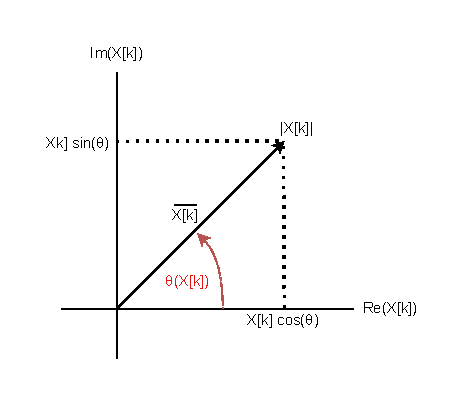
\includegraphics[clip, trim=0 0 0 0, width=0.8\textwidth]{Sections/7_SystemDesign/Figures/7_3_2_DFTUnderstand1.pdf}
    \caption{The fourier coefficient X[k] consists of contributions from both cosines and sine waves. These are the projections of $\vec{X[k]}$ on the real and imaginary axis.}
    \label{fig:7_3_2_DFTU1}
\end{figure}

The sine and cosine components of X[k] on figure \refq{fig:7_3_2_DFTU1} together describe how much of the k'th frequency is present in the sampled input signal and how it is phase shifted relative to the cosine. The magnitude, $|X[k]|$, is the strength of each frequency in the signal, while the phases of each frequency in the signal is $\theta[k]$. The sizes of the sines and cosines components describes how much a signal aligns with the reference cosine or the sine. If the imaginary part is zero, $Im(X[k]) = 0$,  it means the input signal is in-phase with the reference cosine, i.e, the sampled signal is not phase shifted and X[k] lies on the real axis. If the real part is zero, $Re(X[k]) = 0$, it means the sampled signal is phase shifted 90 degrees relative to the reference cosine and X[k] lies on the imaginary axis.

The fourier coefficient shown on figure \refq{fig:7_3_2_DFTU1} contains both cosine and sine waves and means the input signal is phase shifted by some amount. If both real and imaginary parts are zero it means the frequency $f_k$ is not present in the sampled signal at all. All this can be illustrated with the drawing on figure \refq{fig:7_3_2_DFTU2} that relates the magnitude and phase of the X[k] vector in the complex plane to a time domain signal.

\begin{figure}[H]
    \centering
    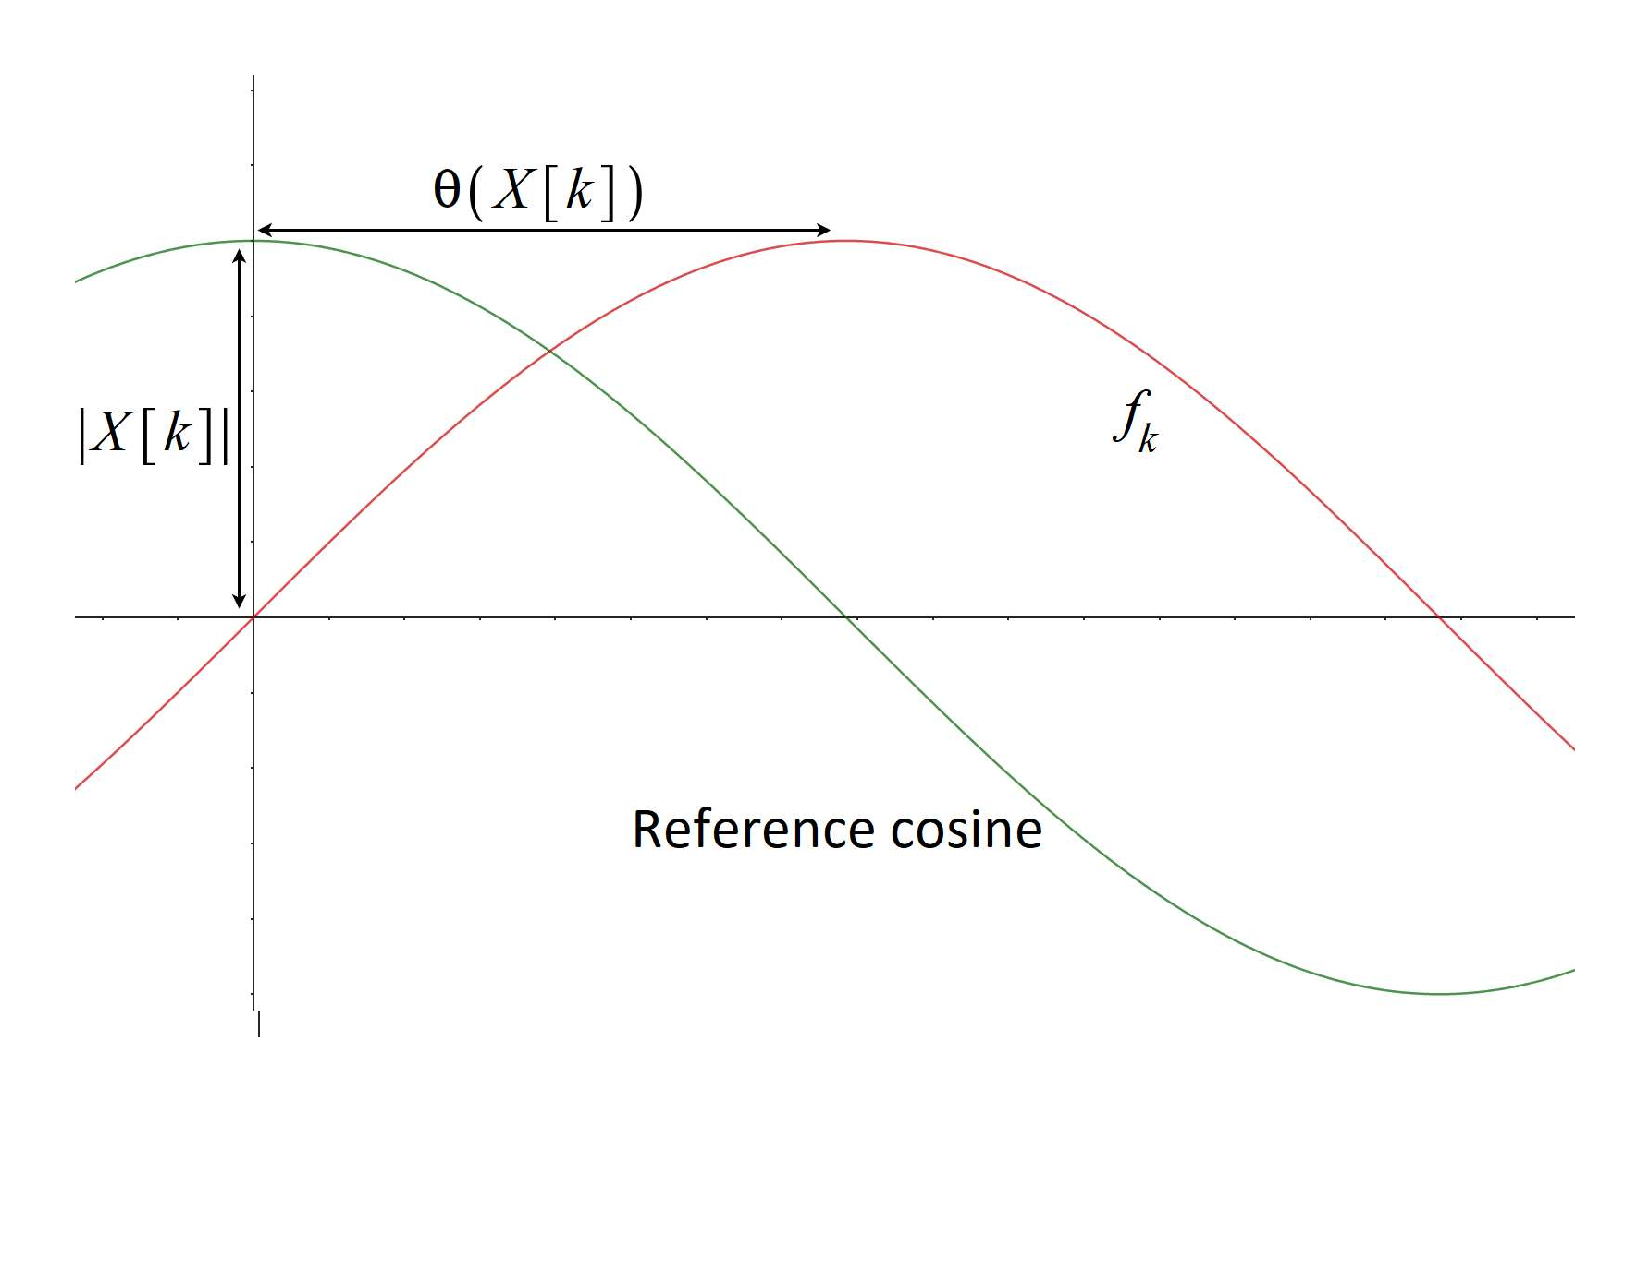
\includegraphics[clip, trim=0 50 0 0, width=0.8\textwidth]{Sections/7_SystemDesign/Figures/7_3_2_DFT_TIME.pdf}
    \caption{The fourier coefficient X[k] consists of contributions from both cosines and sine waves. Depending on the amount of contributions from sine waves it means that the sampled time domain signal has been phase shifted. The magnitude, $|X[k]|$ corresponds to the amplitude of the time domain signal. The signal on the drawing, $f_k$, is but one component of the full time domain signal derived from the X[k]'th fourier coefficient.}
    \label{fig:7_3_2_DFTU2}
\end{figure}

Performing DFT on the voltage and currents will provide both amplitude and phase information about the sampled signals, as shown in figure \refq{fig:7_3_2_DFTU2} and the discussion above, and the fourier coefficients can be used to calculate the DUTs impedance.

Note how both the voltage and current waveform phases are calculated as shown on figures \refq{fig:7_3_2_DFTU2} and \refq{fig:7_3_2_DFTU1}. The reason these phases can be used to calculated the phase of the impedance, is because both the voltage and current waveform is sampled simultaneusly and is thus phased relative to the same reference cosine.

The DFT in eq \refq{eq:4_7_2_SA2} has been implemented as two separate functions in C. The product inside the sum of eq \refq{eq:4_7_2_SA2} is computed in one function, while another function does the summing. The function that computes the product of the input sample, x[n], and exponential term can be seen in listing \refq{lst:DFT_PART_SUM}.

\lstinputlisting[language=C ,style = c,firstnumber=1, linerange=1189-1202, caption={The C function that computes a part-sum of the DFT}, label={lst:DFT_PART_SUM}]{Appendix/Code/main_2612.tex}. 

The function in listing \refq{lst:DFT_PART_SUM} returns a 'complexr' data type. This is a custom data type that can hold a complex number on rectangular form as shown with the type definition on listing \refq{lst:COMPLEXR}.

\lstinputlisting[language=C ,style = c,firstnumber=1, linerange=101-104, caption={A type definition of a complex number.}, label={lst:COMPLEXR}]{Appendix/Code/main_2612.tex}. 

The angle for the complex number is computed in line 5 of listing \refq{lst:DFT_PART_SUM} and this angle is used to compute the real and imaginary parts of the fourier coeffiecient in line 6-8 of listing \refq{lst:DFT_PART_SUM}. The result is stored in the 'fourierPartCoeff' variable and returned to the calling function in line 13.

The CalSingleSampleFourierContribution() function is called by another DFT related function that will retrieve a sample from the external sample memory, check if the sample is a voltage, or current, and then pass it on to CalSingleSampleFourierContribution(). The returned complex number from CalSingleSampleFourierContribution() is summed up into the fourier coefficient X[k] as shown on figure \refq{fig:7_3_2_DFT1}.
\begin{figure}[H]
    \centering
    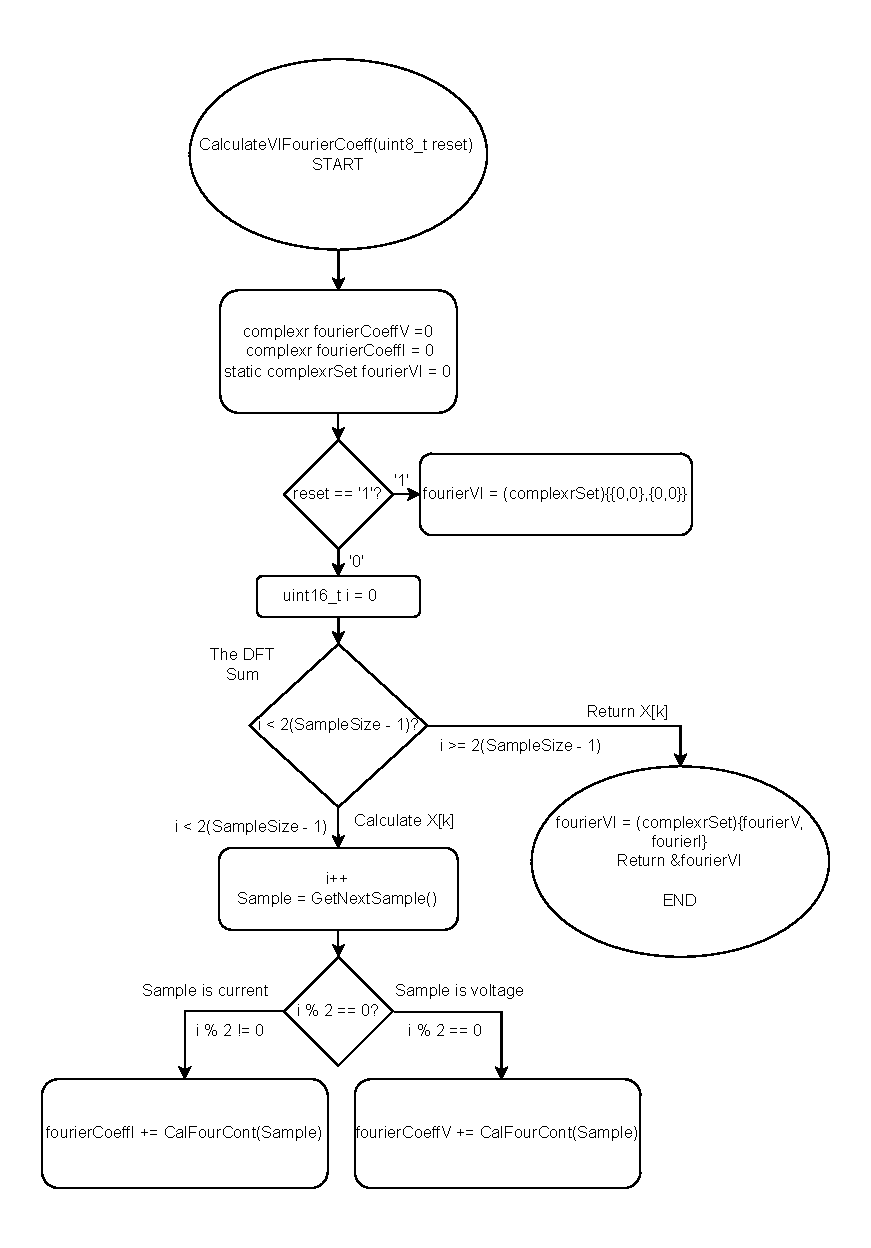
\includegraphics[clip, trim=0 0 0 0, width=0.8\textwidth]{Sections/7_SystemDesign/Figures/7_3_2_DFTFunction.pdf}
    \caption{A flow chart describing the process that calculates the DFT. A number of variables is reset at program start. The fourierV and fourierI will be calculated in the function and saved in the fourierVI variable. The second decision point is the start of the DFT sum and will run to $2(N-1)$ and the reason for this will be described below. The function checks if the sample is a voltage or current sample and computes the DFT part sum on those samples and keeps doing this until it reaches $2(N-1)$ calculations. The function saves the DFT values inside the fourierI and fourierV complex numbers and packs them into a set of complex numbers (complexrSet) and returns a pointer to this set of complex numbers.}
    \label{fig:7_3_2_DFT1}
\end{figure}

The code for the CalculateVIFourierCoeff() function shown on the flow diagram can be found in lines 1149-1187 in the code listing in appendix \refq{App:MCUCode}.
The functions performs the summing function from eq \refq{eq:4_7_2_SA2} and returns a pointer to a set of complex numbers, one for current and one for voltage to the caller. This set of voltage and current fourier coefficients can be used to compute the impedance of the DUT. 

When the function enters the 'for' loop it will retrieve a sample from the sample control module by calling the GetNextSample() function. This function switches the communcation between the MCU and FPGA to the "external memory mode" and returns a sample from the external memory at each function call, starting at address 0.

The function checks if the counting variable $i$ is an even or odd number in order to determine if the sample it has retrieved from the external memory in the Sample Control module is a voltage or current sample. This has to do with the way samples are stored in the memory, as described in section \refq{subsec:PSC}, where a voltage is stored in address 0, followed by a current at address 1 and so on. The function determines if the $i$ variable is an even, or odd, number by dividing it by 2 and checking if there is a remainder or not.

The function returns a pointer to a 'complexrSet' data type variable that can hold two complex numbers, one for voltage and one for current as shown in listing \refq{lst:COMPLEXRSET}.

\lstinputlisting[language=C ,style = c,firstnumber=1, linerange=105-107, caption={A type definition for a set of complex numbers.}, label={lst:COMPLEXRSET}]{Appendix/Code/main_2612.tex}. 

The standard output of the DFT algorithm shown in eq \refq{eq:4_7_2_SA2} is \textit{double-sided} where the frequency spectrum is symmetric around $f_s / 2$, or Nyquist, frequency. This DFT gives $N$ frequency bins, with half of them representing positive frequencies, $f = [0, f_s/2]$ and the other half representing negative frequencies$f = [0, -f_s/2]$.

The negative frequencies are just mirror images, or aliases, of the positive frequencies. Only the positive frequencies are of interest to the project, so the DFT could be converted to a single-sided DFT, by only considering the frequencies in $f = [0, f_s/2]$. To give correct magnitude information the magnitude should be scaled accordingly. The double-sided coefficients can be converted to single-side by removing all content above the sampling frequency, $f > f_s /2$, and multiplying all coefficients under the sampling frequency, $f < f_s /2$, with 2 as shown in \refq{eq:4_7_2_SA8}.

\begin{equation}\label{eq:4_7_2_SA8}
    |X[k]_{scaled}| = 2 \cdot |X[k]|
\end{equation}

The coefficients in eq \refq{eq:4_7_2_SA8} could be normalized with the sample size, so it gives the amplitude of the signal component $f_k$ as shown in eq \refq{eq:4_7_2_SA9}.
\begin{equation}\label{eq:4_7_2_SA9}
    |X[k]_{scaled}| = 2 \cdot \frac{|X[k]|}{N}
\end{equation}

This may be necessary if the voltage and current signals were analyzed independently, but in the end the fourier coefficients for the voltage and current samples will be used to calculate the impedance of the DUT. Impedance is a ratio of voltage and current, $Z = \frac{V}{I}$, so any scaling of the V and I fourier coefficients would cancel and it is thus not necessary for the impedance analysis.
